% Exam Template Probability and Statistics courses
%
% Using Philip Hirschhorn's exam.cls: http://www-math.mit.edu/~psh/#ExamCls
%
% run pdflatex on a finished exam at least three times to do the grading table on front page.
%
%%%%%%%%%%%%%%%%%%%%%%%%%%%%%%%%%%%%%%%%%%%%%%%%%%%%%%%%%%%%%%%%%%%%%%%%%%%%%%%%%%%%%%%%%%%%%%

% These lines can probably stay unchanged, although you can remove the last
% two packages if you're not making pictures with tikz.
\documentclass[12pt,addpoints]{exam}

    % \printanswers   %    <=========  Comment this to print exam without answers
    \newcommand{\gradingnote}[1]{}
    %\newcommand{\gradingnote}[1]{\hfill {\color{red} \textit{Grading note: } #1}}
    
    \newboolean{addsolutionspace}
    \setboolean{addsolutionspace}{true}




\RequirePackage{amssymb, amsfonts, amsmath, latexsym, verbatim, xspace, setspace}
\RequirePackage{tikz, graphicx}
\usepackage{color}
\usepackage{multirow, hhline, array, arydshln, blkarray, subcaption, graphicx, multicol}
\usepackage{txfonts}
\usepackage{hhline, bigstrut}
\usepackage[spanish, es-tabla]{babel}
\usepackage[debug,randomize,nokeeplast]{exam-randomizechoices}
\setrandomizerseed{999}


%\usepackage{calculator, calculus}
\usepackage{soul}
\usetikzlibrary{patterns, plotmarks}
\usepackage{hyperref}
\usepackage{enumerate}
\usepackage{pgfplots, pgfplotstable}
\usepackage[normalem]{ulem}
\useunder{\uline}{\ul}{}

% By default LaTeX uses large margins.  This doesn't work well on exams; problems
% end up in the "middle" of the page, reducing the amount of space for students
% to work on them.
\usepackage[margin=1in]{geometry}

\newboolean{hasattachment}\setboolean{hasattachment}{false}
\newboolean{openbook}\setboolean{openbook}{false}
\newboolean{opennotes}\setboolean{opennotes}{false}
\newboolean{calculator}\setboolean{calculator}{false}


%\newcommand\openbooktrue{\setboolean{openbook}{true}}

%patch the exam package and change the format of the grade table.
\usepackage{etoolbox}
\makeatletter
\patchcmd{\questions}
  {\def\@currentlabel{\thequestiontitle}}
  {\def\@currentlabel{\thequestion}}
  {}
  {}
\makeatother

% ======================================
		% Here's where you edit the Class, Exam, Date, etc.
		\newcommand{\career}{Ingeniería Biomédica}
		\newcommand{\term}{Primer Semestre de 2024}
		\newcommand{\classcode}{PSIM} 
		\newcommand{\codeOfCurseA}{81}
		\newcommand{\formajor}{\quad Procesamiento de Señales e Imágenes}
		\newcommand{\examnum}{Examen Final}
		\newcommand{\examdate}{21/05/24}
		\newcommand{\timelimit}{\quad 60 Minutos} 
		\newcommand{\weight}{20}
		\newcommand{\numberpage}{3}
		\newcommand{\numberquestion}{9}
		\newcommand{\numberpoint}{100} 
		\newcommand{\classtitle}{Procesamiento de Señales e Imágenes Médicas}
		\newcommand{\class}{\classcode -- \classtitle}
		\newcommand{\classShort}{\classcode}



%1. La **teoría de wavelet** es un campo matemático que se ocupa del análisis de señales.
%2. Las **wavelets** son funciones matemáticas que cortan datos en diferentes componentes de frecuencia y luego estudian cada componente con una resolución que coincide con su escala.
%3. Son útiles para la **compresión de datos** y la **reducción de ruido**.
%4. Una wavelet es una onda que tiene una duración limitada, lo que significa que tiene un valor de cero en todas partes excepto en un intervalo pequeño.
%5. Las wavelets pueden ser usadas para descomponer funciones o señales en componentes más pequeños.
%6. Esta descomposición permite un análisis más detallado de la información local en la señal.
%7. Las wavelets son particularmente útiles cuando los datos que estás analizando tienen un número de características diferentes a diferentes escalas.
%8. En términos matemáticos, una wavelet es una función que puede ser usada para dividir una función o señal en diferentes componentes de frecuencia.
%9. Las wavelets son útiles en una variedad de aplicaciones, incluyendo la compresión de imágenes, la eliminación de ruido en señales de audio y la detección de patrones en datos financieros.
%10. La transformada de wavelet es una herramienta que te permite ver cómo cambian las frecuencias de una señal con el tiempo.
%11. Las wavelets son una alternativa a las transformadas de Fourier para el análisis de señales.
%12. A diferencia de las transformadas de Fourier, que descomponen una señal en sinusoides de diferentes frecuencias, las wavelets descomponen una señal en pequeñas ondas de diferentes frecuencias.
%13. Esto significa que las wavelets son capaces de proporcionar información sobre la frecuencia y la ubicación de una característica en una señal.
%14. La teoría de wavelet ha sido aplicada en una variedad de campos, desde la física hasta la ingeniería y la informática.
%15. Las wavelets son especialmente útiles en el procesamiento de señales digitales, donde permiten un análisis eficiente y flexible de las señales.
%16. La teoría de wavelet también ha encontrado aplicaciones en la compresión de datos, donde puede ser usada para reducir la cantidad de datos necesarios para representar una señal sin perder mucha información.
%17. En resumen, las wavelets son una herramienta poderosa para el análisis de señales que proporciona una forma flexible y eficiente de descomponer señales en componentes de diferentes frecuencias.
%18. La teoría de wavelet es un campo de estudio en constante evolución con muchas aplicaciones potenciales.
%19. Las wavelets son una herramienta valiosa en cualquier campo que requiera el análisis de señales o datos.
%20. En última instancia, la teoría de wavelet es una forma de entender cómo las diferentes partes de una señal o conjunto de datos interactúan entre sí a diferentes escalas. 


% **Transformada de Fourier**
% 1. La **Transformada de Fourier** es una herramienta matemática utilizada para descomponer funciones periódicas en una suma de funciones sinusoidales simples.
% 2. Es una técnica fundamental en el procesamiento de señales y la física.
% 3. La Transformada de Fourier convierte una señal del dominio del tiempo al dominio de la frecuencia.
% 4. Permite analizar las diferentes frecuencias presentes en una señal.
% 5. Es útil para el análisis espectral y la filtración de señales.
% 6. La Transformada de Fourier puede ser discreta (DFT) o continua (FT).
% 7. La DFT se utiliza comúnmente en el procesamiento digital de señales.
% 8. La FT se utiliza en señales continuas y es fundamental en la física cuántica.
% 9. La Transformada de Fourier inversa (IFT) se utiliza para reconstruir la señal original a partir de su espectro de frecuencia.
% 10. La Transformada de Fourier es una operación lineal e invertible.

% **Transformada de Gabor**
% 11. La **Transformada de Gabor** es una transformada que combina la Transformada de Fourier con una ventana temporal.
% 12. Fue desarrollada por Dennis Gabor, quien recibió el Premio Nobel de Física por este trabajo.
% 13. La Transformada de Gabor es útil para el análisis de señales no estacionarias, es decir, señales cuyas propiedades estadísticas cambian con el tiempo.
% 14. Proporciona información tanto en el dominio del tiempo como en el dominio de la frecuencia, lo que se conoce como una representación tiempo-frecuencia.
% 15. La Transformada de Gabor utiliza una función de ventana, que puede ser cualquier función que sea cero fuera de un intervalo.
% 16. La función de ventana se desplaza a lo largo de la señal, y en cada posición se aplica la Transformada de Fourier.
% 17. Esto da como resultado una serie de espectros de frecuencia a corto plazo, que muestran cómo cambia el contenido de frecuencia de la señal con el tiempo.
% 18. La Transformada de Gabor es útil en muchas aplicaciones, incluyendo el procesamiento de voz y de imágenes.
% 19. La Transformada de Gabor es una operación lineal e invertible.
% 20. La Transformada de Gabor inversa se utiliza para reconstruir la señal original a partir de su representación tiempo-frecuencia.

	
		%% == comment the following lines if needed
		\hasattachmenttrue  
		% \openbooktrue
		% \opennotestrue
		\calculatortrue
% ======================================

% For an exam, single spacing is most appropriate
\singlespacing
% \onehalfspacing
% \doublespacing

% For an exam, we generally want to turn off paragraph indentation
\parindent 0ex

\everymath{\displaystyle}

\pointpoints{punto}{puntos}
\hpword{Puntos:}
\vpword{Puntos}
\htword{Totale}
\vtword{Totale:}
\vsword{Resultado}

\begin{document}
% These commands set up the running header on the top of the exam pages
\pagestyle{head}
\firstpageheader{PSIM Primer Parcial}{}{Page 1 of 5}
\firstpageheadrule
\runningheader{ID: }{\classcode\ \ \examnum\ \ (\examdate)}{Page \thepage\ of \numpages}
\runningheadrule
\begin{minipage}[t]{0.6\textwidth}
\hspace{-0.1em}

\includegraphics[scale=0.15]{Uni_logo.png}
\end{minipage}%
\begin{minipage}[t]{0.4\textwidth}
	\vspace*{-2.8cm}
	\begin{tabular}{l p{0.5in}}
		\textbf{Nombre:} & \makebox[1.5in]{\hrulefill} \\
		\\
		\textbf{Código:} & \makebox[1.5in]{\hrulefill} \\
		\\
		\textbf{Curso:} & \makebox[1.5in]{\hrulefill} \\
		\\
	\end{tabular}
\end{minipage}


%	\rule[1ex]{\textwidth}{.1pt}

	\begin{center}
	\begin{Large}
		\textbf{\career}
	\\ \bigskip
    \textbf{\class}
    \\ \bigskip
    \textbf{\examnum -- \examdate}	
	\\ \bigskip
	\term
    \\ \bigskip
    \end{Large}
	\end{center}

	\makebox[1.2in][l]{\textbf{Línea de énfasis:}}  \fbox{\parbox[c][1em][l]{0.79\textwidth}{\textbf{\formajor}}}   \smallskip
	\bigskip
	
	\makebox[1.2in][l]{\textbf{Fecha:}} \fbox{\parbox[c][1em][l]{0.8in}{\ \examdate}}  	\hfill
	\makebox[1.6in][l]{\textbf{Duración:}} \fbox{\parbox[c][1em][l]{1.4in}{\ \timelimit}}  	
	\bigskip\smallskip
	
	
	\makebox[0.8in][l]{\textbf{Porcentaje:}} \fbox{\parbox[c][1em][l]{0.3in}{\ \weight}}\%  	\qquad
	\makebox[0.8in][l]{\textbf{No. Pág:}} \fbox{\parbox[c][1em][l]{0.2in}{\ \numberpage}}    \hfill	
	\makebox[1in][l]{\textbf{No. Preg:}} \fbox{\parbox[c][1em][l]{0.2in}{\ \numberquestion}}  	\qquad
	\makebox[1in][l]{\textbf{Tot. de ptos:}} \fbox{\parbox[c][1em][l]{0.3in}{\ \numberpoint}}  	
	\bigskip
	\bigskip
	
\centering	{\Large\textbf{\underline{Instrucciones:}}}\smallskip
\begin{table}[h]
\centering
\parbox{0.3\textwidth}{
\begin{tabular}{lll}
\multicolumn{3}{c}{{\ul Solo para uso del profesor:}} \\
 &  &  \\
\begin{tabular}[c]{@{}l@{}}Pregunta \\ Número\end{tabular} & \begin{tabular}[c]{@{}l@{}}Total\\ Marks\end{tabular}  & \multicolumn{1}{r}{Score} \\
 &  &  \\ \hline
\multicolumn{1}{|l|}{1} & \multicolumn{1}{l|}{} & \multicolumn{1}{l|}{} \\ \hline
\multicolumn{1}{|l|}{2} & \multicolumn{1}{l|}{} & \multicolumn{1}{l|}{} \\ \hline
\multicolumn{1}{|l|}{3} & \multicolumn{1}{l|}{} & \multicolumn{1}{l|}{} \\ \hline
\multicolumn{1}{|l|}{4} & \multicolumn{1}{l|}{} & \multicolumn{1}{l|}{} \\ \hline
\multicolumn{1}{|l|}{5} & \multicolumn{1}{l|}{} & \multicolumn{1}{l|}{} \\ \hline
\multicolumn{1}{|l|}{6} & \multicolumn{1}{l|}{} & \multicolumn{1}{l|}{} \\ \hline
\multicolumn{1}{|l|}{7} & \multicolumn{1}{l|}{} & \multicolumn{1}{l|}{} \\ \hline
\multicolumn{1}{|l|}{8} & \multicolumn{1}{l|}{} & \multicolumn{1}{l|}{} \\ \hline
\multicolumn{1}{|l|}{9} & \multicolumn{1}{l|}{} & \multicolumn{1}{l|}{} \\ \hline
\multicolumn{1}{|l|}{10} & \multicolumn{1}{l|}{} & \multicolumn{1}{l|}{} \\ \hline
\multicolumn{1}{|l|}{11} & \multicolumn{1}{l|}{} & \multicolumn{1}{l|}{} \\ \hline
\multicolumn{1}{|l|}{Total} & \multicolumn{1}{l|}{} & \multicolumn{1}{l|}{} \\ \hline
\end{tabular}
}
\begin{minipage}[c]{0.6\textwidth}%
	\begin{scriptsize}
		\begin{enumerate}
		\item Escriba su nombre, su código y el código del curso (\codeOfCurseA) en el \textbf{extremo superior derecho} de esta página. Además marque cada hoja con su nombre en el campo Nombre de cada hoja (\textbf{esquina superior izquierda}).
		\item Responad todas las preguntas en el espacio apropiado. Si se lo exige, escriba la mayor cantidad de explicaciones posible, de esto dependerá el número de puntos otorgados.
		\item Preguntas sin responder se les dará \textbf{CERO (0)} puntos.
		\item Este es un examen con \textbf{MATERIAL ABIERTO}. Sin embargo, TODO el material debe estar escrito con su puño y letra.
		\item Se \textbf{permite} calculadoras.
		\item No se permite el uso de celulares.
		\item No se permite compartir ningún tipo de material, ni producto de papelería.
		\item N.A. significa ninguna de las anteriores. No confundir con NAN que significa ''not a number´´.
		\end{enumerate}
	\end{scriptsize}
\end{minipage}
\end{table}

%%%%%%%%%%%%%%%%%%%%%%%%%
%
%  questions 
\pgfplotsset{compat=1.17}
%
%%%%%%%%%%%%%%%%%%%%%%%%%
\begin{questions}
%\qformat{Pregunta \thequestion: \thequestiontitle\dotfill\thepoints}
\qformat{{\qquad \bf Pregunta \thequestion}: \ \  [\totalpoints \ puntos] \hfill}
%\qformat{{\bf Problem \thequestion}: \ \  [\thepoints] \hfill}


\begin{scriptsize}
	\titledquestion{}
	\begin{figure}
		\begin{subfigure}{0.4\textwidth}
			\centering
			
\includegraphics[width=\textwidth]{pregFourier1.png} %for multiple choice question
			\caption{Espectro de Magnitud. Pregunta 1A \label{pregunta1A}}
		\end{subfigure}
		\hfill
		\begin{subfigure}{0.4\textwidth}
			\centering
			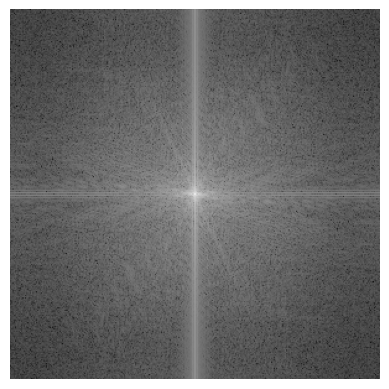
\includegraphics[width=\textwidth]{pregFourier2.png} %for multiple choice question
			\caption{Espectro de Magnitud. Pregunta 1B \label{pregunta1B}}
		\end{subfigure}
		\begin{subfigure}{0.4\textwidth}
			\centering
			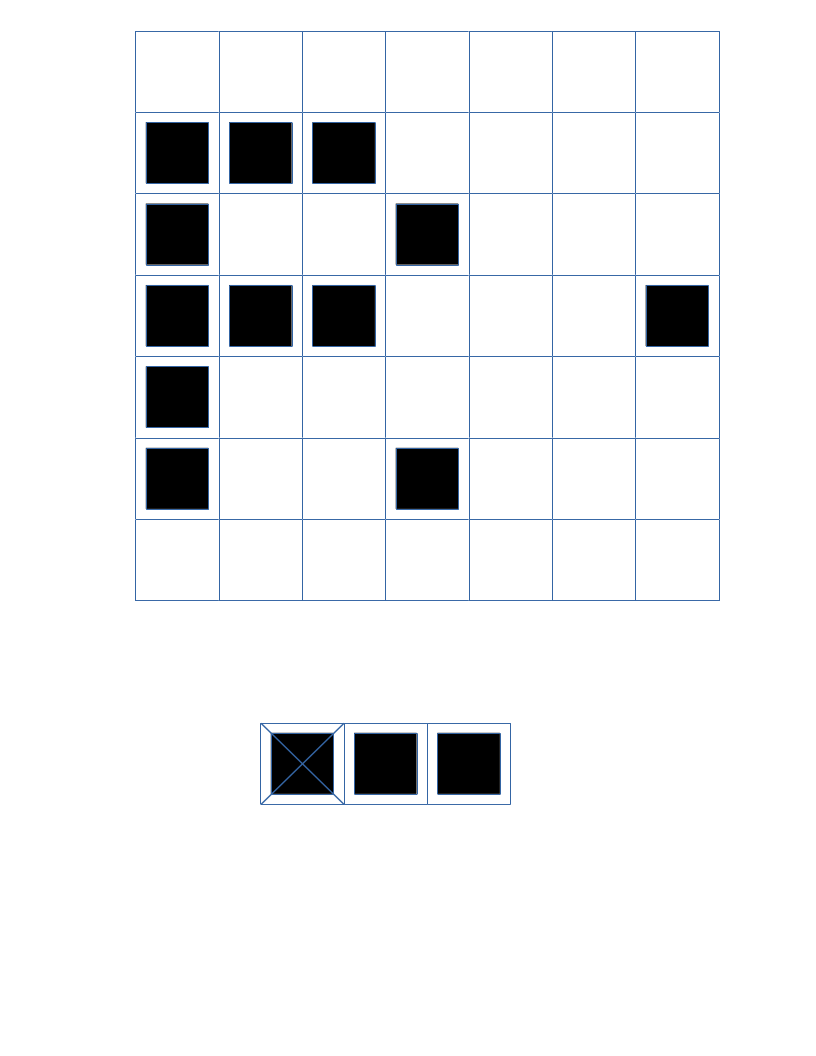
\includegraphics[width=\textwidth]{Morfologia.png} 
			\caption{Imagen binaria \label{pregunta2e}}
		\end{subfigure}
		\hfill
		\begin{subfigure}{0.4\textwidth}
			\centering
			
\includegraphics[width=\textwidth]{Respuesta.png}
			\caption{Espacio para la respuesta \label{pregunta2eRTA}}
		\end{subfigure}
	\end{figure}	

	\begin{multicols}{2}
		
        \begin{parts}
				\part[5] En la Figura \ref{pregunta1A}, se presenta un espectro de magnitud para una imagen desconocida. Cuales de las siguientes afirmaciones son correctas:\newline
        		\begin{checkboxes}
        			\choice La resolución de la imagen es de 70x70.
        			\choice La imagen tiene solo variaciones de intensidad lumínica verticales.
        			\choice La imagen tiene solo variaciones de intensidad lumínica horizontales.
					\choice La imagen puede presentar variaciones de intensidad lumínica parásitas, debidas al fenómeno de Gibbs.
        			\choice Ninguna de las respuestas es verdadera.
        		\end{checkboxes}
                
            \part[5] En la Figura \ref{pregunta1B}, se observa un espectro de magnitud de una imagen desconocida. Cuales de las siguientes afirmaciones son correctas? \newline
			\begin{checkboxes}
				\choice La resolución espacial de la imagen es desconocida.
				\choice Las variaciones de la intensidad luminica verticales son mayores que las horizontales.
				\choice La imagen se asemeja a un tablero de ajedrez donde se intercalan puntos blancos y negros.
				\choice Ninguna de las respuestas es verdadera.
			\end{checkboxes}

			\part[5] "La transformación de Fourier es muy útil porque permite porque permite el procesamiento de señales no homosedásticas". Esta frase es: \newline
			\begin{checkboxes}
				\choice Verdadera porque la transformación de Fourier de una señal ubica los cambios de frecuencias, sin el uso de ninguna operación extra de procesamiento. 
				\choice Verdadera pero solo para cambios puntuales en la variabilidad de la señal y solo si se usa en conjunto con una estrategia de ventaneo de la señal. 
				\choice Falsa porque la transformación de Fourier no calcula variaciones en frecuencia.
				\choice Falsa porque la transformación de Fourier no calcula TODAS las alteraciones de la variabilidad de la señal.
				\choice Ninguna de las respuestas es válida.
			\end{checkboxes}

			\part[5] Cual(es) de las siguientes afirmaciones es(son) correctas \newline
        		\begin{checkboxes}
        			\choice En la transformada corta de Fourier se hace un compromiso en el análisis frecuencial a favor de un realizar un análisis temporal básico.
        			\choice La transformada de Fourier permite la ubicación de cualquier cambio abrupto o discontinuidad en la señal.
        			\choice La transformada de Fourier solo procesa señales no estacionarias
					\choice Una señal estacionaria no tiene cambios en su variabilidad en el total de su duración.
        			\choice Todas las afirmaciones son falsas.
        		\end{checkboxes}

        \end{parts}
            

	\titledquestion{}
        \begin{parts}
			\part[5] "La transformada Wavelet es un operación donde se obtiene una descomposición de la señal". Cual o Cuales de las siguientes afirmaciones responde mejor a la veracidad de la anterior frase:
            \smallskip
            \newline
        		\begin{checkboxes}
        			\choice Es verdadera porque toma la señal y calcula coeficientes de senos y cosenos; los cuales corresponden a las componentes de señal.
        			\choice Es falsa porque no todas las señales se pueden integrar.
        			\choice Es verdadera porque con esta transformacion se calculan los componetes de una señal basandose en funciones de energía finita de duración limitada.
        			\choice Es falsa porque esa transformación no existe.
					\choice todas las demas respuestas no son viables.
        		\end{checkboxes}

				\part[5] Se desea hacer el análisis de la variabilidad de ritmo cardíaco. Cual(es) de los siguientes procedimientos son los más apropiados para cumplir esta tarea.
				\smallskip
				\newline
					\begin{checkboxes}
						\choice Tomo el ECG y hago un filtro pasa altas de 60Hz porque a esta frecuencia se encuentra el ritmo cardíaco medio.
						\choice Tomo el ECG y le aplico una transformación de Fourier dado que esta operación calcula las variaciones en frecuencia.
						\choice Tomo el ECG y le aplico una transfomación de Wavelet con una wavelet madre tipo db4 para poder estudiar los cambios de variabilidad.
						\choice Tomo el EMG y le aplico una transfomación de Wavelet con una wavelet madre tipo db4 para poder estudiar los cambios de variabilidad.
						\choice Ninguno de los procedimientos es válido.
					\end{checkboxes}

					\part[5] En la transformada Wavelet, la función de escalamiento es:
					\smallskip
					\newline
						\begin{checkboxes}
							\choice La función de escalamiento no existe
							\choice La función de escalamiento es el factor que más influye en la localización tiempo-frecuencia. 
							\choice La función de escalamiento es especialmente útil en el análisis de señales no estacionarias.
							\choice En el análisis multiresolución la función de escalamiento es determinada por los procesos de submuestreos (downsampling) sucesivos.
							\choice Ninguna de las otras afirmaciones es válida
						\end{checkboxes}

					\part[5] En el análisis multiresolución, el banco de filtros depende de la función de escalamiento.
					\smallskip
					\newline
						\begin{checkboxes}
							\choice Falso
							\choice Verdadero
						\end{checkboxes}

					\part[10] En la figura~\ref{pregunta2eRTA}, grafique la salida de una operación de dilatación con la información de la figura~\ref{pregunta2e}
					\smallskip
					\newline
                
        \end{parts}

	\question[10]
		
	\end{multicols}
\end{scriptsize}

\begin{figure}

\end{figure}

\end{questions}
\end{document}

